\documentclass{weekly}
\begin{document}
\maketitlew{Аналитическая механика}{1}{3}{9}

\begin{wrapfigure}[6]{r}{4.5cm}\vspace{-5.5mm}
    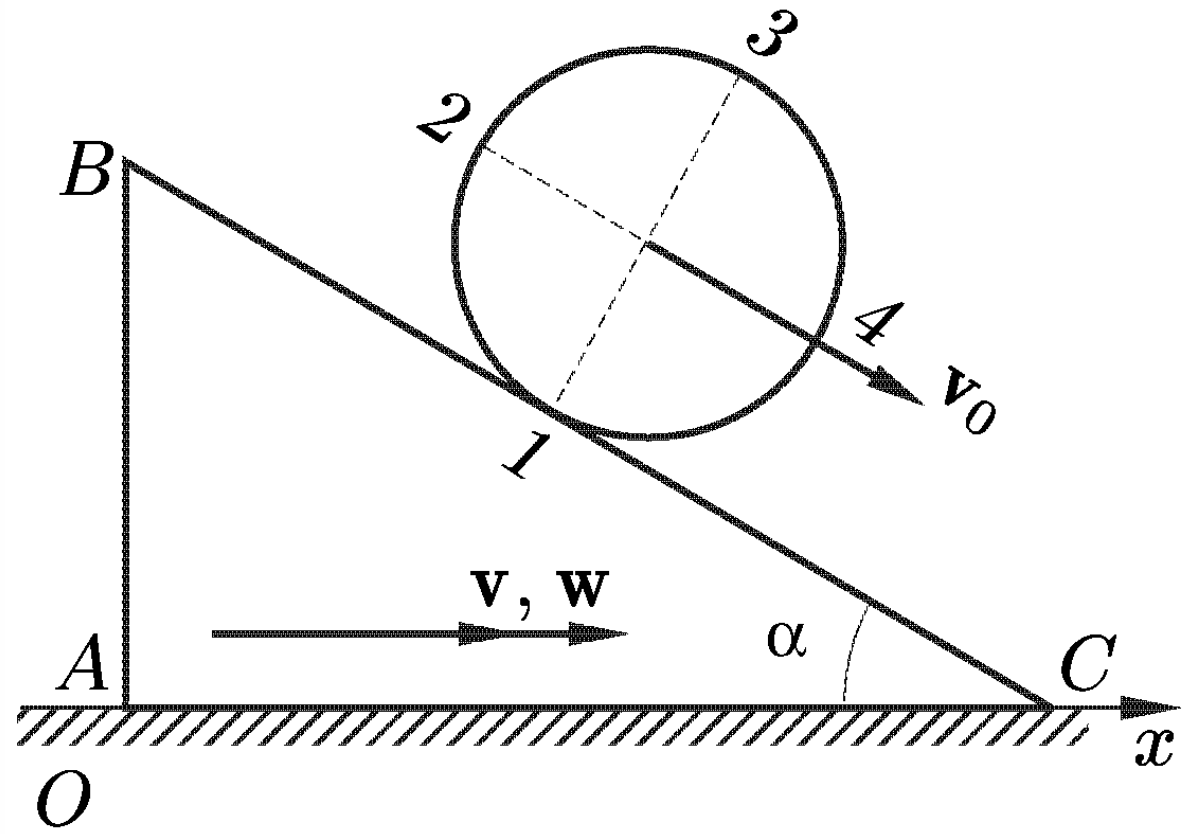
\includegraphics[width=\lw]{2-11}
\end{wrapfigure}
\paragraph{2.11.} Призма~$ABC$ движется поступательно вдоль~оси~$Ox$
с~ускорением~$\vec{w}$, имея в~данный момент скорость~$\vec{v}$.
По~линии наибольшего ската~$BC$ призмы катится без~скольжения
цилиндр, скорость центра которого относительно призмы постоянна
и~равна~$\vec{v_0}$. Радиус цилиндра~$R$, $\angle BCA = \alpha$.
Найти скорости и~ускорения точек~$1, 2, 3, 4$ цилиндра
в~данный момент времени.

$\blacktriangleright$ В~подвижной (штрихованной) системе отсчёта призмы
цилиндр совершает мгновенное вращение вокруг точки~$1$:
$\vec v'_1 = \overline{0}$.
Введём координатные оси: направление~$Ox$ уже задано, $Oy$ направим
вертикально вверх, $\hat z = \hat x \times \hat y$.
\emph{Без~доказательства} заявим, что угловая скорость цилиндра
\begin{equation}
    \vec\omega = -\frac{v_0}{R} \hat z.
\end{equation}

Скорости всех заданных точек найдутся по~формуле Эйлера
($\vec v'_i = \vec\omega \times \vec r_{1i}$):
\begin{align}
    \vec v'_2 &= -\frac{v_0}{R} \hat z \times
            \cvec{\sqrt{2} R\sin\left(\alpha - \frac{\pi}{4}\right)}
            {\sqrt{2} R\cos\left(\alpha - \frac{\pi}{4}\right)}{0}
        = \sqrt{2} v_0
            \left[ \cos\left(\alpha - \frac{\pi}{4}\right) \hat x
            - \sin\left(\alpha - \frac{\pi}{4}\right) \hat y \right]; \\
    \vec v'_3 &= -\frac{v_0}{R} \hat z \times
            \cvec{2R\sin\alpha}{2R\cos\alpha}{0}
        = 2v_0 \left[ \cos\alpha \cdot \hat x -
            \sin\alpha \cdot \hat y \right]; \\
    \vec v'_4 &= -\frac{v_0}{R} \hat z \times
            \cvec{\sqrt{2} R\sin\left(\alpha + \frac{\pi}{4}\right)}
            {\sqrt{2} R\cos\left(\alpha + \frac{\pi}{4}\right)}{0}
        = \sqrt{2} v_0
            \left[ \cos\left(\alpha + \frac{\pi}{4}\right) \hat x
            - \sin\left(\alpha + \frac{\pi}{4}\right) \hat y \right].
\end{align}

Переход к~неподвижной системе отсчёта осуществляется легко и~приятно:
$\vec v_i = \vec v'_i + \vec v$.
\begin{align}
    \vec v_1 &= v \hat x, & \label{2.11:v1}
        v_1 &= v; \\
    \vec v_2 &= \cvec{v + v_0 (\cos\alpha + \sin\alpha)}
            {v_0 (\cos\alpha - \sin\alpha)}{0}, & \label{2.11:v2}
        v_2 &= \sqrt{v^2 + 2v_0^2 +
            2vv_0 (\cos\alpha + \sin\alpha)}; \\
    \vec v_3 &= \cvec{v + 2v_0 \cos\alpha}{-2v_0 \sin\alpha}{0}, &
        \label{2.11:v3}
        v_3 &= \sqrt{v^2 + 4v_0^2 + 4vv_0 \cos\alpha}; \\
    \vec v_4 &= \cvec{v + v_0 (\cos\alpha - \sin\alpha)}
            {-v_0 (\sin\alpha + \cos\alpha)}{0} & \label{2.11:v4}
        v_4 &= \sqrt{v^2 + 2v_0^2 + 2vv_0 (\cos\alpha - \sin\alpha)}.
\end{align}

Ускорение центра цилиндра в~штрихованной системе равно нулю.
Значит, $\vec w'_i = \vec\omega \times \vec\omega \times \vec r_{0i}$:
\begin{align}
    \vec w'_1 &= -\omega^2 R \left[ -\sin\alpha \cdot \hat x -
            \cos\alpha \cdot \hat y \right]; \\
    \vec w'_2 &= -\omega^2 R \left[ -\cos\alpha \cdot \hat x +
            \sin\alpha \cdot \hat y \right]; \\
    \vec w'_3 &= -\omega^2 R \left[ +\sin\alpha \cdot \hat x +
            \cos\alpha \cdot \hat y \right]; \\
    \vec w'_4 &= -\omega^2 R \left[ +\cos\alpha \cdot \hat x -
            \sin\alpha \cdot \hat y \right].
\end{align}
Аналогично, поскольку призма движется поступательно, всё очень приятно:
\begin{align}
    \vec w_1 &= \cvec{w + v_0^2/R \cdot \sin\alpha}
            {v_0^2/R \cdot \cos\alpha}{0}, & \label{2.11:w1}
        w_1 &= \sqrt{w^2 + \frac{v_0^4}{R^2} +
            \frac{2wv_0^2}{R}\sin\alpha}; \\
    \vec w_2 &= \cvec{w + v_0^2/R \cdot \cos\alpha}
            {-v_0^2/R \cdot \cos\alpha}{0}, & \label{2.11:w2}
        w_2 &= \sqrt{w^2 + \frac{v_0^4}{R^2} +
            \frac{2wv_0^2}{R}\cos\alpha}; \\
    \vec w_3 &= \cvec{w - v_0^2/R \cdot \sin\alpha}
            {-v_0^2/R \cdot \cos\alpha}{0}, & \label{2.11:w3}
        w_3 &= \sqrt{w^2 + \frac{v_0^4}{R^2} -
            \frac{2wv_0^2}{R}\sin\alpha}; \\
    \vec w_4 &= \cvec{w - v_0^2/R \cdot \cos\alpha}
            {-v_0^2/R \cdot \sin\alpha}{0}, & \label{2.11:w4}
        w_4 &= \sqrt{w^2 + \frac{v_0^4}{R^2} -
            \frac{2wv_0^2}{R}\cos\alpha}.
\end{align}

\textbf{Ответ:}\quad \eqref{2.11:v1}~-- \eqref{2.11:v4}, ~
\eqref{2.11:w1}~-- \eqref{2.11:w4}.
\hfill $\blacktriangleleft$

\end{document}
